\subsubsection{Varnish}
\label{soa:tecnologias:varnish}

\gls{db:varnish} es un proxy reverso HTTP, a veces referenciado como HTTP accelerator o a web accelerator.  Un proxy reverso es un servidor proxy que recupera recursos desde uno o mas servidores.  Estos recursos se devuelven al cliente como si se hubieran originado desde el propio servidor proxy, es decir, actúa como intermediario entre los clientes y servidores.
Varnish almacena archivos y framentos de archivos en memoria, lo que reduce el tiempo de respuestea y el ancho de banda de red para las mismas solicitudes.\cite[p.~20]{varnish2016}

El proyecto fue iniciado en el 2005 por el Noruego Verdens Gang, el arquitecto y desarrollador principal es el consultor danés Poul Henning Kamp, desarrollador del núcleo de FreeBSD. El proyecto además contó con el gerencia, infraestructura y desarrollos adicionales aportados por la comunidad Noruega de Linux, Linpro. El soporte, gerencia y desarrollo luego paso a una empresa independiente, Varnish Software.

Dependiendo de su instalación, varnish puede ser usado para:

\begin{itemize}
  \item web application firewall,
  \item DDoS attack defender,
  \item load balancer,
  \item integration point,
  \item single sign-on gateway,
  \item authentication and authorization policy mechanism,
  \item quick fix for unstable backends, and
  \item HTTP router
\end{itemize}

Como mencionamos anteriormente, \gls{db:varnish} es un acelerador de aplicaciones web, que se instala delante de cualquier servidor HTTP y se configura para almacenar en la caché del servidor una copia del recurso solicitado. Pensado para mejorar el rendimiento de aplicaciones web con contenidos pesados y APIs altamente consumidas.

Actualmente es utilizado por una gran cantidad de sitios web con alta demanda de tráfico como pueden ser: The New York Times, The Guardian, The Hindu, Corriere della Sera, y sitios de redes sociales y contenidos como Wikipedia, Facebook, Twitter, Vimeo, Tumblr, entre otros. De los top 10K sitios en la web, alrededor de una décima parte usan Varnish Cache.


\begin{figure}[H]
  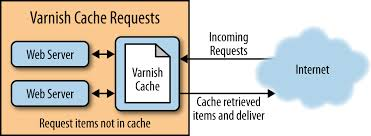
\includegraphics[width=\linewidth]{src/images/03-capitulo-3/tecnologias/varnish/reverse-proxy.jpg}
  \caption{Varnish Reverse Proxy}
  \label{fig:varnish}
\end{figure}

\paragraph{Licencia}

Varnish Cache es software libre, licenciado bajo una licencia BSD

\paragraph{Instalación y prueba}

\begin{listing}[H]
  \bashfile{src/03-capitulo-3/tecnologias/cache/code/varnish/00-preparacion.sh}
  \caption{Instalación de Varnish}
  \label{soa:tecnologias:varnish-cache:bash-preparacion}
\end{listing}
